\documentclass{beamer}

\usepackage[utf8]{inputenc}
\usepackage[T1]{fontenc}

\usepackage{bibentry}
\usepackage{graphicx}
\usepackage{booktabs}
\usepackage[portuguese]{babel}
\usepackage{comment}
\usepackage{xcolor}
\usepackage{enumitem}
\usepackage{hyperref}
\usepackage[normalem]{ulem}


\setbeamertemplate{caption}[numbered]
\usetheme{Darmstadt}

\definecolor{vim-green}{rgb}{0.004, 0.596, 0.200}
\colorlet{beamer@blendedblue}{green!40!black}

\newenvironment{wideitemize}{\itemize\addtolength{\itemsep}{2em}}{\enditemize}
\newenvironment{widedescription}{\description\addtolength{\itemsep}{2em}}{\enddescription}
\newcommand{\key}[1]{\colorbox{lightgray}{\textbf{#1}}}
\newcommand{\sk}[1]{\textless #1\textgreater}
\newcommand{\bk}[1]{\{#1\}}

%Information to be included in the title page:
\title{Minicurso Vim}
\author{André William Régis \\ Pedro Santi Binotto}
\institute{UFSC}
\date{\the\year}

\begin{document}

\frame{\titlepage}
\section{Introdução}

\begin{frame}{Material de apoio}
    \fbox{
        \parbox{\linewidth}{
        \$ git clone --recursive \\ https://github.com/AndreKuru/Minicurso-Vim.git
        }
    }

    \vfill

    \hyperlink{https://media.pragprog.com/titles/dnvim2/code/dnvim2-code.zip}{pratical-vim-examples}
\end{frame}

\begin{frame}{Vim}
    \begin{columns}
        \begin{column}{0.3\textwidth}
            \begin{figure}
                \centering
                
\includegraphics[height=0.6\linewidth]{Image/vi-logo.png}
                \label{vi-logo}
            \end{figure}
        \end{column}
        
        \begin{column}{0.3\textwidth}
            \begin{figure}
                \centering
                
\includegraphics[height=0.6\linewidth]{Image/vim-logo.png}
                \label{vim-logo}
            \end{figure}
        \end{column}
        
        \begin{column}{0.3\textwidth}
            \begin{figure}
                \centering
                
\includegraphics[height=0.6\linewidth]{Image/neovim-logo.png}
                \label{neovim-logo}
            \end{figure}
        \end{column}
        
    \end{columns}
\end{frame}

\begin{frame}{Principais modos}
    \begin{wideitemize}
        \item \textbf{Normal}: navegar e editar
        \item \textbf{Insert}: inserção de texto
        \item \textbf{Visual}: editar através de seleção
        \item \textbf{Command-line}: retentor de usuários de primeira viagem
    \end{wideitemize}
\end{frame}

\begin{frame}{Digitação ideal}
    \begin{figure}
        \centering
        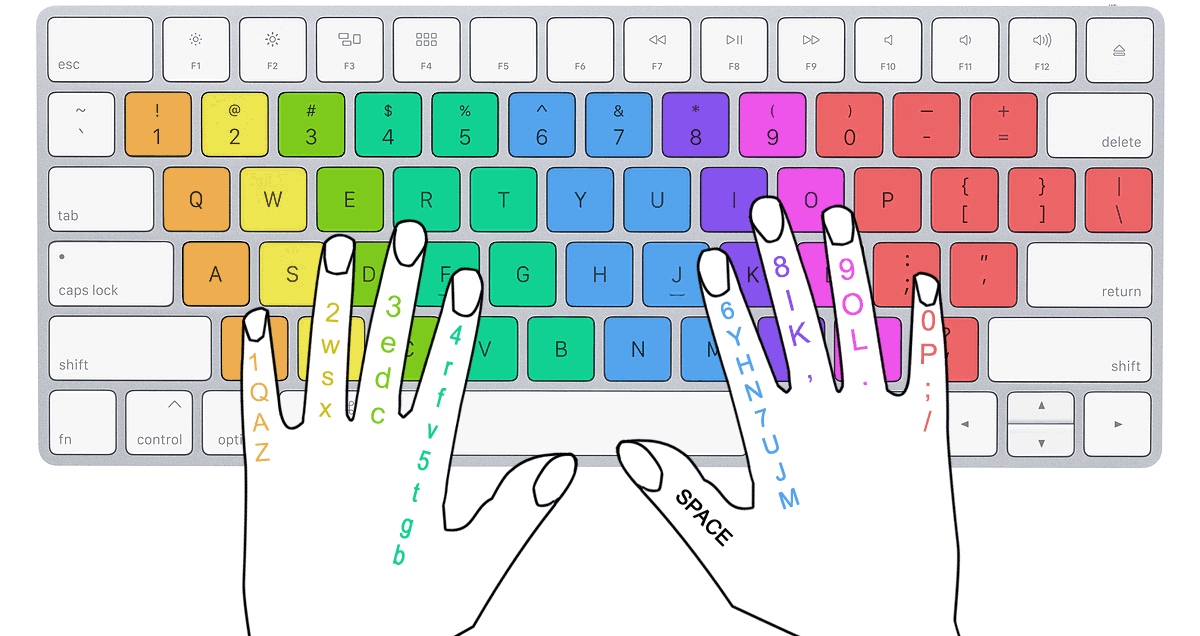
\includegraphics[width=\linewidth]{Image/Finger_position_on_a_keyboard.png}
        \label{finger-position}
        \footnotesize
        \\ Imagem não adaptada. \\
        Disponível em:  \hyperlink{https://commons.wikimedia.org/wiki/File:Finger_position_on_a_keyboard.png}{Wikimedia}
    \end{figure}
\end{frame}


\begin{frame}{Movimentação básica}
    \begin{columns}
        \begin{column}{0.4\textwidth}
            \begin{widedescription}
                \item \key{j}: $\downarrow$
                \item \key{k}: $\uparrow$
                \item \key{l}: $\rightarrow$
                \item \key{h}: $\leftarrow$
                \item Jogo para praticar: \\ \hyperlink{https://vim-adventures.com/}{vim-adventures.com}
            \end{widedescription}
        \end{column}
        
        \begin{column}{0.6\textwidth}
            \begin{figure}
                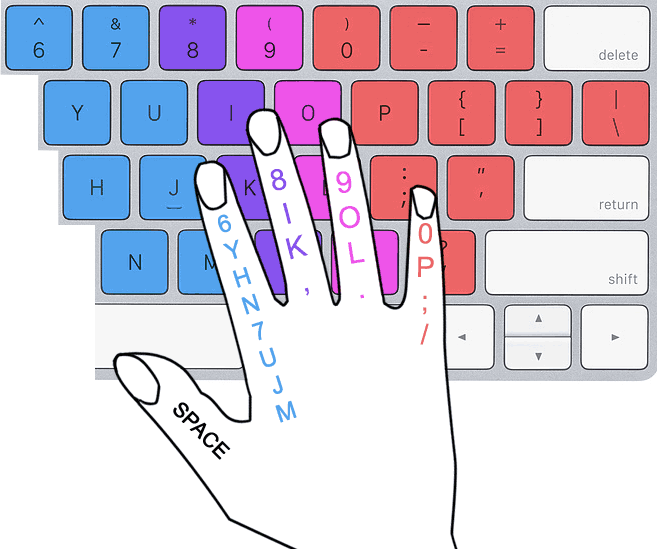
\includegraphics[width=\linewidth]{Image/Finger_position_on_a_keyboard-only-right-hand.png}
                \label{right-hand} 
                \footnotesize
                \\ Imagem adaptada. \\
                Disponível em:  \hyperlink{https://commons.wikimedia.org/wiki/File:Finger_position_on_a_keyboard.png}{Wikimedia}
            \end{figure}
        \end{column}
    \end{columns}

    \begin{flushleft}
    \end{flushleft}
\end{frame}

\begin{frame}{Quando não se precisa manter a mão no mouse}
    \begin{columns}
        \begin{column}{0.4\linewidth}
            \begin{wideitemize}
                \item \key{u}: \textbf{u}ndo change
                \item \key{dd}: \textbf{d}elete line
                \item \key{yy}: \textbf{y}ank line
                \item \key{p}: \textbf{p}ut text
            \end{wideitemize}
        \end{column}
        
        \begin{column}{0.3\textwidth}
            \begin{figure}
                
\includegraphics[width=\linewidth]{Image/kelly-sikkema-K5dAn1gOFEc-unsplash.jpg}
                \footnotesize
                \\ Imagem não adaptada. \\
                Disponível em:  \hyperlink{https://unsplash.com/photos/person-using-black-and-silver-laptop-computer-K5dAn1gOFEc}{Unsplash}
            \end{figure}
        \end{column}
        
        \begin{column}{0.3\textwidth}
            \begin{widedescription}
                \item Mas se quiser pode
                \item \key{:set mouse=a}
            \end{widedescription}
        \end{column}
    \end{columns}
\end{frame}

\begin{frame}{Experimentando cada modo}
    \begin{wideitemize}
        \item \key{i}: switch to \textbf{I}nsert mode
        \item \key{v}: switch to \textbf{V}isual mode
        \item \key{:}: switch to Command-Line mode
    \end{wideitemize}
\end{frame}

\begin{frame}{Como sair do vim?}
    \begin{widedescription}
        \item \key{:q}: \textbf{q}uit
        \item \key{:q!}: \textbf{q}uit without writing
        \item \key{:w}: \textbf{w}rite
        \item \key{:wq}: \textbf{w}rite and \textbf{q}uit
        \item \key{:x}: write (if needed) and quit
    \end{widedescription}
\end{frame}
\section{Normal}
\begin{frame}{Comando ponto}
    \begin{widedescription}
    \centering
        \item \key{.}: "Repeat last change [...]"
    \end{widedescription}
\end{frame}

\begin{frame}{Mudanças comuns}
    \begin{columns}
        \begin{column}{0.5\textwidth}
            \begin{widedescription}
                \item \key{x}: delete [count] char(s)
                \item \key{s}: \textbf{s}ubstitute [count] char(s)
                \item \key{[]}: "[...] are optional."
                \item \key{[count]}: "An optional number that may precede the command to multiply or iterate the command."
            \end{widedescription}
        \end{column}
        
        \begin{column}{0.5\textwidth}
            \begin{widedescription}
                \item \key{d\bk{motion}}: \textbf{d}elete
                \item \key{c\bk{motion}}: \textbf{c}hange
                \item \key{\bk{}}: "[...] must appear, but which can take a number of different values."
                \item \key{\bk{motion}}:  "A command that moves the cursor."
            \end{widedescription}
        \end{column}
    \end{columns}
\end{frame}

\begin{frame}{Movimentação na linha}
    \begin{widedescription}
        \item \key{0}: start of the line
        \item \key{\$}: end of the line
        \item \key{\^{}}: start non-blank of the line
        \item \key{g\_}: end non-blank of the line
    \end{widedescription}
\end{frame}

\begin{frame}{Movimentação através de palavras}
    \begin{columns}
        \begin{column}{0.4\textwidth}
            \begin{widedescription}
                \item \key{w}: \textbf{w}ord foward
                \item \key{e}: word \textbf{e}nd foward
                \item \key{b}: word \textbf{b}ackward
                \item \key{ge}: word end backward
            \end{widedescription}
        \end{column}
        
        \begin{column}{0.6\textwidth}
            \begin{widedescription}
                %\item \textbf{word}: [A - z], [0 - 9] and \_
                \item \textbf{word}: "[...] \\ letters, digits and underscores, \\
                or a sequence of other non-blank characters [...]"
                \item \textbf{blank characters}: "space and tab"
            \end{widedescription}
        \end{column}
    \end{columns}
\end{frame}

\begin{frame}{Movimentação através de PALAVRAS}
    \begin{columns}
        \begin{column}{0.4\textwidth}
            \begin{widedescription}
                \item \key{W}: \textbf{W}ORD foward
                \item \key{E}: WORD \textbf{e}nd foward
                \item \key{B}: WORD \textbf{b}ackward
                \item \key{gE}: WORD end backward
            \end{widedescription}
        \end{column}
        
        \begin{column}{0.6\textwidth}
            \begin{widedescription}
                \item \textbf{WORD}: "[...] \\ sequence of non-blank characters [...]"
                \item \textbf{blank characters}: "space and tab"
            \end{widedescription}
        \end{column}
    \end{columns}
\end{frame}

\begin{frame}{Buscas dentro da linha}
    \begin{columns}
        \begin{column}{0.3\textwidth}
            \begin{widedescription}
            \item \key{f}: \textbf{f}ind char \\ to the right
            \item \key{t}: \textbf{t}ill before char \\ to the right
            \item \key{F}: \textbf{f}ind char \\ to the left
            \item \key{T}: \textbf{t}ill after char \\ to the left
            \end{widedescription}
        \end{column}

        \begin{column}{0.7\textwidth}
           \begin{widedescription}
               \item \key{;}: "Repeat latest f, t, F or T [...]"
               \item \key{,}: "Repeat latest f, t, F or T \\ in opposite direction [...]"
           \end{widedescription} 
        \end{column}
    \end{columns}
\end{frame}

\begin{frame}{Buscas no arquivo}
    \begin{columns}
        \begin{column}{0.4\textwidth}
            \begin{widedescription}
            \item \key{/}: search forward for the pattern
            \item \key{?}: search backward for the pattern
            \item \key{*}: search forward for the nearest word
            \item \key{\#}: search backward for the nearest word
            \end{widedescription}
        \end{column}

        \begin{column}{0.6\textwidth}
           \begin{widedescription}
               \item \key{n}: "Repeat latest "/" or "?" [...]"
               \item \key{N}: "Repeat latest "/" or "?" \\ in opposite direction [...]"
           \end{widedescription} 
        \end{column}
    \end{columns}
\end{frame}

\begin{frame}{Operadores}
    \begin{columns}
        \begin{column}{0.5\textwidth}
            \begin{widedescription}
                \item \key{c}: \textbf{c}hange
                \item \key{d}: \textbf{d}elete
                \item \key{y}: \textbf{y}ank
                \item \key{\textgreater}: shift right
                \item \key{\textless}: shift left
            \end{widedescription}
        \end{column}
        
        \begin{column}{0.5\textwidth}
            \begin{widedescription}
                \item \key{=}: autoident
                \item \key{g\~}: swap case
                \item \key{gu}: make lowercase
                \item \key{gU}: make uppercase
                %\item \key{!}: Filter \{motion\} lines through an external program
            \end{widedescription}
        \end{column}
    \end{columns}
\end{frame}

%\begin{frame}{Comandos condensados}
%    \begin{columns}
%        \begin{column}{0.5\textwidth}
%            \begin{widedescription}
%                \item \key{C} = \key{c\$}
%                \item \key{s} = \key{cl}
%                \item \key{S} = \key{\^{}C}
%            \end{widedescription}
%        \end{column}
%        
%        \begin{column}{0.5\textwidth}
%            \begin{widedescription}
%                \item \key{I} = \key{\^{} i}
%                \item \key{A} = \key{\$a}
%                \item \key{o} = \key{A\sk{CR}}
%                \item \key{O} = \key{ko}
%            \end{widedescription}
%        \end{column}
%    \end{columns}
%\end{frame}

\begin{frame}{Teclas especiais}
    \begin{columns}
        \begin{column}{0.35\textwidth}
            \begin{widedescription}
                \item \key{\sk{Enter}}: Enter
                \item \key{\sk{Esc}}: Escape
                \item \key{\sk{S-...}}: Shift + ...
                \item \key{\sk{A-...}}: Alt + ...
                \item \key{\sk{C-...}}: Ctrl + ...
            \end{widedescription}
        \end{column}
        
        \begin{column}{0.65\textwidth}
            \begin{widedescription}
                \item \key{\sk{CR}}: Carriage Return
                \item \key{\sk{Up}}: Up arrow key
                \item \key{\sk{S-Down}}: Shift + Down arrow key
                \item \key{Ctrl-A}: Ctrl + a
                \item \key{\sk{C-x}}: Ctrl + x
            \end{widedescription}
        \end{column}
    \end{columns}
\end{frame}

\begin{frame}{Aritmética simples}
    \begin{widedescription}
        \item \key{\sk{C-a}}: \textbf{a}dd [count] to the number at or after the cursor
        \item \key{\sk{C-x}}: subtract [count] to the number at or after the cursor
    \end{widedescription}
\end{frame}

\section{Inserção}
\begin{frame}{Nem tudo se transforma}
    \begin{columns}
        \begin{column}{0.6\textwidth}
            \begin{widedescription}
                \item \key{i}: \textbf{i}nsert text
                \item \key{a}: \textbf{a}ppend text
                \item \key{I}: \textbf{i}nsert text at the start of the line
                \item \key{A}: \textbf{a}ppend text at the end of the line
            \end{widedescription}
        \end{column}
        
        \begin{column}{0.4\textwidth}
            \begin{widedescription}
                \item \key{o}: \textbf{o}btain new line below
                \item \key{O}: \textbf{o}btain new line above
            \end{widedescription}
        \end{column}
    \end{columns}
\end{frame}

\begin{frame}{Correções rápidas}
    \begin{widedescription}
        \item \key{\sk{C-h}}: delete back one character (\key{\sk{BS}})
        \item \key{\sk{C-w}}: delete back one \textbf{w}ord
        \item \key{\sk{C-u}}: delete back to the start of line
    \end{widedescription}
\end{frame}

\begin{frame}{Transições}
    \begin{widedescription}
        \item \key{\sk{Esc}}: switch to Normal mode
        \item \key{\sk{C-[}}: switch to Normal mode
        \item \key{\sk{C-o}}: switch to Insert Normal mode
    \end{widedescription}
\end{frame}

\begin{frame}{Acessar registradores}
    \begin{widedescription}
        \item \key{\sk{C-r}\bk{register}}: "Insert the contents of a register."
        \item \key{\bk{register}}:
        \begin{description}
            \item \key{+}:	the clipboard contents
            \item \key{*}:	the clipboard contents (X11: primary selection)
            \item \key{0}: contains the text from the most recent yank command
            \item \key{1-9}: contains the text deleted in ascending order by \\ the most recent delete or change command
            \item \key{=}: the expression register
        \end{description}
    \end{widedescription}
\end{frame}

\begin{frame}{Inserir caracteres por código}
    \begin{columns}
        \begin{column}{0.6\textwidth}
            \begin{widedescription}
                \item \key{\sk{C-v}191}: ¿
                \item \key{\sk{C-v}u00bf}: ¿
                \item \key{\sk{C-v}u00b0}: °
                \item \key{\sk{C-v}\{nondigit\}}: e.g. \key{\sk{Home}}
            \end{widedescription}
        \end{column}
        
        \begin{column}{0.42\textwidth}
            \begin{widedescription}
                \item \key{\sk{C-k}\bk{char1}\bk{char2}}
                \item \key{\sk{C-k}?I}: ¿
                \item \key{\sk{C-k}12}: ½
                \item \key{ga}: print the ascii value
            \end{widedescription}
        \end{column}
    \end{columns}
\end{frame}

\begin{frame}{Mais um modo}
    \begin{widedescription}
        \item \key{R}: \textbf{R}eplace mode
        \item \key{gR}: Virtual \textbf{R}eplace mode
        \item \key{r}: \textbf{r}eplace single character
        \item \key{gr}: virtual \textbf{r}eplace single character
    \end{widedescription}
\end{frame}
\section{Visual}

\begin{frame}{Cada modo uma orientação}
    \begin{columns}
        \begin{column}{0.55\textwidth}
            \begin{widedescription}
                \item \key{v}: switch character-wise \\ \textbf{V}isual mode
                \item \key{V}: switch line-wise \\ \textbf{V}isual Line mode
                \item \key{\sk{C-v}}: switch block-wise \\ \textbf{V}isual Block mode
            \end{widedescription}
        \end{column}
        
        \begin{column}{0.45\textwidth}
            \begin{widedescription}
                \item \key{\sk{Esc}}: switch to Normal mode
                \item \key{\sk{C-[}}: switch to Normal mode
                \item \key{gv}: re-select last \\ \textbf{v}isual selection
                \item \key{o}: go to \textbf{o}ther \\ end of selected text
            \end{widedescription}
        \end{column}
    \end{columns}
\end{frame}

\begin{frame}{Seleção entre delimitadores}
    \begin{columns}
        \begin{column}{0.6\textwidth}
            \begin{widedescription}
                \item \key{a)} or \key{ab}: \textbf{a} pair of \textbf{(}parentheses\textbf{)}
                \item \key{a\}} or \key{aB}: \textbf{a} pair of \{braces\}
                \item \key{a'}: \textbf{a} pair of \textbf{'}single quotes\textbf{'}
                \item \key{a"}: \textbf{a} pair of \textbf{"}\textbf{"}double quotes\textbf{"}
            \end{widedescription}
        \end{column}
        
        \begin{column}{0.4\textwidth}
            \begin{widedescription}
                \item \key{a]}: \textbf{a} pair of \textbf{[}brackets\textbf{]}
                \item \key{a\textgreater}: \textbf{a} pair of \textbf{\textless\textgreater}
                \item \key{a`}: \textbf{a} pair of \textbf{`}backticks\textbf{`}
                \item \key{at}: \textbf{a} pair of \textbf{t}ags
            \end{widedescription}
        \end{column}
    \end{columns}
\end{frame}

\begin{frame}{Seleção entre delimitadores}
    \begin{columns}
        \begin{column}{0.6\textwidth}
            \begin{widedescription}
                \item \key{i)} or \key{ib}: \textbf{i}nside of \textbf{(}parentheses\textbf{)}
                \item \key{i\}} or \key{iB}: \textbf{i}nside of \{braces\}
                \item \key{i'}: \textbf{i}nside of \textbf{'}single quotes\textbf{'}
                \item \key{i"}: \textbf{i}nside of \textbf{"}double quotes\textbf{"}
            \end{widedescription}
        \end{column}
        
        \begin{column}{0.4\textwidth}
            \begin{widedescription}
                \item \key{i]}: \textbf{i}nside of \textbf{[}brackets\textbf{]}
                \item \key{i\textgreater}: \textbf{i}nside of \textbf{\textless\textgreater}
                \item \key{i`}: \textbf{i}nside of \textbf{`}backticks\textbf{`}
                \item \key{it}: \textbf{i}nside of \textbf{t}ags
            \end{widedescription}
        \end{column}
    \end{columns}
\end{frame}

\begin{frame}{Seleção de objeto}
    \begin{columns}
        \begin{column}{0.5\textwidth}
            \begin{widedescription}
                \item \key{aw}: \textbf{a}round of \textbf{w}ord
                \item \key{aW}: \textbf{a}round of \textbf{W}ORD
                \item \key{as}: \textbf{a}round of \textbf{s}entence
                \item \key{ap}: \textbf{a}round of \textbf{p}aragraph
            \end{widedescription}
        \end{column}
        
        \begin{column}{0.5\textwidth}
            \begin{widedescription}
                \item \key{iw}: \textbf{i}nside of \textbf{w}ord
                \item \key{iW}: \textbf{i}nside of \textbf{W}ORD
                \item \key{is}: \textbf{i}nside of \textbf{s}entence
                \item \key{ip}: \textbf{i}nside of \textbf{p}aragraph
            \end{widedescription}
        \end{column}
    \end{columns}
\end{frame}


% \section{Linha de comando}

\begin{frame}{Falando do ex}
    \begin{widedescription}
        \item \key{:print}: print current line
        \item \key{:3print}: print line 3
        \item \key{:2,4print}: print lines 2 to 4
        \item \key{:'\textless ,'\textgreater print}: print lines selected from visual mode
    \end{widedescription}
\end{frame}

\begin{frame}{Comandos básicos}
    \begin{columns}
        \begin{column}{0.45\linewidth}
            \begin{widedescription}
                \item \key{:[range]print}
                \item \key{:[range]join}
                \item \key{:[range]copy \bk{address}}
                \item \key{:[range]move \bk{address}}
            \end{widedescription}
        \end{column}
        
        \begin{column}{0.56\textwidth}
            \begin{widedescription}
                \item \key{[range]}: \key{\bk{address}[,\bk{address}]}
                \item \key{\bk{address}}: 
                    \small
                    \begin{description}
                        \item \key{number}: absolute line number
                        \item \key{.}: current line
                        \item \key{\$}: last line in the file
                        \item \key{\%}: current file
                        \item \key{/\bk{pattern}[/]}: next line [...]
                        \item \key{?\bk{pattern}[?]}: previous line [...]
                    \end{description}
            \end{widedescription}
        \end{column}
    \end{columns}
\end{frame}

\begin{frame}{Comandos básicos}
    \begin{columns}
        \begin{column}{0.5\linewidth}
            \begin{widedescription}
                \item \key{:[range]delete [x]}
                \item \key{:[range]yank [x]}
                \item \key{:[range]put [x]}
            \end{widedescription}
        \end{column}
        
        \begin{column}{0.5\textwidth}
            \begin{widedescription}
                \item \key{[x]}: "[into register x]"
                \begin{description}
                    \item \key{a},\key{b},\key{c},\key{d},\key{e},\key{f},\key{g},\key{h}, \\
                    \item \key{i},\key{j},\key{k},\key{l},\key{m},\key{n},\key{o},\key{p}, \\
                    \item \key{q},\key{r},\key{s},\key{t},\key{u},\key{v},\key{w},\key{x}, \\
                    \item \key{y},\key{z} \end{description}
            \end{widedescription}
        \end{column}
    \end{columns}
\end{frame}

\begin{frame}{Os mais populares}
    \begin{widedescription}
        \item \key{:[range]normal \bk{address}}
        \item \key{:[range]substitute/\bk{pattern}/\bk{string}/[flags]}
        \item \key{:[range]global/\bk{pattern}/[cmd]}
        \item \key{[cmd]}: command from command line
    \end{widedescription}
\end{frame}

\begin{frame}{Repetição é a chave}
    \begin{widedescription}
        \item \key{@:}: execute the last ex command
        \item \key{@@}: execute the last \key{@}
        \item \key{@\bk{register}}: execute the contents of register
        \item \key{q}: record/stop macro
    \end{widedescription}
\end{frame}

\begin{frame}{Comandos externos}
    \begin{widedescription}
        \item \key{:shell}: start shell
        \item \key{:!\bk{cmd}}: execute \key{\bk{cmd}} in the shell
    \end{widedescription}
\end{frame}

\begin{frame}{Comandos externos integrados com o arquivo atual}
    \begin{widedescription}
        \item \key{:read !\bk{cmd}}: execute \key{\bk{cmd}} in the shell \\ and put the output as text below cursor
        \item \key{:[range]write !\bk{cmd}}: execute \key{\bk{cmd}} in the shell \\ with \key{[range]} lines as input
        \item \key{:[range] !\bk{filter}}: execute \key{\bk{cmd}} in the shell \\ and put the output as text below cursor \\ with \key{[range]} lines as input
    \end{widedescription}
\end{frame}
% \section{Extra}

\begin{frame}{Rolar texto}
    \begin{columns}
        \begin{column}{0.5\linewidth}
            \begin{widedescription}
                \item \key{\sk{C-E}}: scroll window \\ (\textbf{E}xtra lines)
                \item \key{\sk{C-D}}: scroll window \\ \textbf{D}onwards
                \item \key{\sk{C-F}}: scroll window \\ \textbf{F}orwards
            \end{widedescription}
        \end{column}
        \begin{column}{0.5\linewidth}
            \begin{widedescription}
                \item \key{\sk{C-Y}}: scroll window \\ (\textbf{Y}rineu)
                \item \key{\sk{C-U}}: scroll window \\ \textbf{U}pwards
                \item \key{\sk{C-B}}: scroll window \\ \textbf{B}ackwards
            \end{widedescription}
        \end{column}
    \end{columns}
\end{frame}

\begin{frame}{Saltando pelo texto}
    \begin{widedescription}
        \item \key{[count]G}: \textbf{g}o to line number
        \item \key{\%}: jump to matching parenthesis
        \item \key{m\bk{letter}}: set \key{\bk{mark}} \key{\bk{letter}} at cursor position
        \item \key{\`{}\bk{mark}}: jump to a \key{\bk{mark}}
    \end{widedescription}
\end{frame}

\begin{frame}{Navegando pelos saltos}
    \begin{widedescription}
        \item \key{\sk{C-]}}: "Jump to the definition of the keyword under the cursor."
    \end{widedescription}

    \vfill
    
    \begin{columns}
        \begin{column}{0.5\linewidth}
            \begin{widedescription}
                \item \key{\sk{C-o}}: go to \textbf{o}lder \\ cursor position in jump list.
            \end{widedescription}
        \end{column}
        \begin{column}{0.5\linewidth}
            \begin{widedescription}
                \item \key{\sk{C-i}}: go to \sout{\textbf{i}rineu} newer \\ cursor position in jump list.
            \end{widedescription}
        \end{column}
    \end{columns}
\end{frame}

\begin{frame}{Autocomplete}
    \begin{widedescription}
        \item \key{\sk{C-n}}: find \textbf{n}ext match
        \item \key{\sk{C-p}}: find \textbf{p}revious match
    \end{widedescription}
\end{frame}
% \section{Buffers}
\begin{frame}{\textit{Buffers, windows, tabs}}
  \begin{widedescription}
    \item \begin{quotation} \small\it
      Summary: \\
      \hspace{1em} A buffer is the in-memory text of a file. \\
      \hspace{1em} A window is a viewport on a buffer. \\
      \hspace{1em} A tab page is a collection of windows\cite{vimReferenceManual}. \\
    \end{quotation}
  \end{widedescription}
\end{frame}

\begin{frame}{\textit{Buffers} no Vim}
  \begin{widedescription}
    \item A window is a viewport onto a buffer.  You can use multiple windows on one buffer, or several windows on different buffers.
    \item A buffer is a file loaded into memory for editing.  The original file remains unchanged until you write the buffer to the file\cite{vimReferenceManual}.
  \end{widedescription}
\end{frame}

\begin{frame}{\textit{Buffers} no Vim}
  A buffer can be in one of three states:
  \begin{widedescription}
    \item \textbf{active:} The buffer is displayed in a window. If there is a file for this buffer, it has been read 
      into the buffer. The buffer may have been modified since then and thus be different from the file.

    \item \textbf{hidden:} The buffer is not displayed. If there is a file for this buffer, it has been read into the
      buffer. Otherwise it's the same as an active buffer, you just can't see it.

    \item \textbf{inactive:} The buffer is not displayed and does not contain anything. Options for the buffer are
      remembered if the file was once loaded. It can contain marks from the \key{shada} file.  But the buffer
      doesn't contain text\cite{vimReferenceManual}.
  \end{widedescription}
\end{frame}

\begin{frame}{Trabalhando com \textit{buffers}}
  \begin{tabular}{ |p{1.5cm}||p{2cm}|p{1.5cm}|p{2cm}|  }
  \hline
    \multicolumn{4}{|c|}{Buffer states} \\
  \hline
    state & displayed in window & loaded & \key{:buffers} shows\\
  \hline
    active & yes & yes & 'a' \\
    hidden & no & yes & 'h' \\
    inactive & no & no & ' ' \\
  \hline
  \end{tabular}
\end{frame}

\begin{frame}{Trabalhando com \textit{buffers}}
  \begin{widedescription}
    \item \key{:e}:   \textbf{e}dit file
    \item \key{:bn}:  \textbf{b}uffer \textbf{n}ext
    \item \key{:bp}:  \textbf{b}uffer \textbf{p}revious
    \item \key{:bd}:  \textbf{b}uffer \textbf{d}elete
    \item \key{:b[n]}: ex.: \textit{buffer\textbf{1}} \textit{buffer\textbf{2}}
  \end{widedescription}
\end{frame}

\begin{frame}{\textit{Windows}: \textit{viewports} bara \textit{buffers}}
  \begin{widedescription}
    \item \key{:split}:   Divide horizontalmente a tela com uma nova janela; \\
      \key{:split ./outro/arquivo.txt}
    \item \key{:vsplit}:  Divide verticalmente a tela com uma nova janela; \\
      \key{:vsplit ./outro/arquivo.txt}
    \item \key{:close[n]}:   Fecha uma janela (janela ativa ou \key{[n]}); \\
      \key{:close}, \key{:close 1}
  \end{widedescription}
\end{frame}

\begin{frame}{\textit{Windows}: \textit{viewports} bara \textit{buffers}}
  \begin{widedescription}
    \item \key{\sk{C-W}s}:    \key{:split}
    \item \key{\sk{C-W}v}:    \key{:vsplit}
  \end{widedescription}
  \vspace{1cm}
  \textbf{Note:} All \key{CTRL-W} commands can also be executed with \key{:wincmd}, for those places where a Normal
  mode command can't be used or is inconvenient\cite{vimReferenceManual}.
\end{frame}

\begin{frame}{\textit{Windows}: \textit{viewports} bara \textit{buffers}}
  \begin{columns}
    \begin{column}{0.5\linewidth}
      \begin{widedescription}
        \item \key{\sk{C-W}[hjkl]}: Move to window above/below/right of/left of current one.
      \end{widedescription}
    \end{column}
    \begin{column}{0.5\linewidth}
      \begin{widedescription}
        \item \key{\sk{C-W}[HJKL]}: Move window above/below/to the right/to the left.
      \end{widedescription}
    \end{column}
  \end{columns}
  \vspace{1cm}
  \textbf{Note:} All \key{CTRL-W} commands can also be executed with \key{:wincmd}, for those places where a Normal
  mode command can't be used or is inconvenient\cite{vimReferenceManual}.
\end{frame}

\begin{frame}{\textit{Tab-pages}}
  \begin{widedescription}
  \item A tab page holds one or more windows.  You can easily switch between tab
  pages, so that you have several collections of windows to work on different
  things\cite{vimReferenceManual}.
  \end{widedescription}
\end{frame}

\begin{frame}{\textit{Tab-pages}}
  \begin{columns}
    \begin{column}{0.5\linewidth}
      \begin{widedescription}
        \item \key{:tabe}:   \textbf{tab e}dit
        \item \key{:tabnew}: \textbf{tab new}
        \item \key{:tabc}:   \textbf{tab c}lose
      \end{widedescription}
    \end{column}
    \begin{column}{0.5\linewidth}
      \begin{widedescription}
        \item \key{:tabn}:   \textbf{tab n}ext
        \item \key{:tabp}:   \textbf{tab p}revious
        \item \key{:tabs}:   \textbf{tabs} (plural de tab)
      \end{widedescription}
    \end{column}
  \end{columns}
\end{frame}

% \section{Neovim}
\begin{frame}{O sucessor moderno}
    \begin{columns}
        \begin{column}{0.6\textwidth}
            \begin{widedescription}
              \item \begin{quotation} \small\it
                Neovim is exactly what it claims to be. It fixes every issue I have with Vim.\\
                \hspace{1em plus 1fill}---Geoff Greer
              \end{quotation}

              \item \begin{quotation} \small\it
                Full-screen Neovim looks cool as hell!\\
                \hspace{1em plus 1fill}---DHH
              \end{quotation}

              \item \begin{quotation} \small\it
                A nice looking website, that's one thing Neovim did right.\\
                \hspace{1em plus 1fill}---Bram Moolenaar
              \end{quotation}

            \end{widedescription}
        \end{column}

        \begin{column}{0.6\textwidth}
            \begin{figure}
                \centering
                
\includegraphics[height=0.6\linewidth]{Image/neovim-logo.png}
                \label{neovim-logo-1}
                \footnotesize
                \\ Imagem não adaptada. \\
                Disponível em:  \hyperlink{https://neovim.io}{Neovim}
            \end{figure}
        \end{column}
    \end{columns}
\end{frame}

\begin{frame}{O sucessor moderno}
    \begin{widedescription}
        \item API versionada, documentada;
        \item Completamente configurável em Lua; 
        \item Ecossistema extensivo de plugins desenvolvidos pela comunidade; \item Analisador sintático \textit{TreeSitter} permite highlighting e navegação de código a nivel de objetos sintáticos;
        \item Cliente de LSP embutido (mesmo protocolo do \textit{VSCode}!) habilita funcionalidades de inteligência de
          código (refatoração automática, \textit{code actions}, navegação por referência, etc...);
        \item Configuração inicial amigável;
        \item Completamente compatível com Vim original;
    \end{widedescription}
\end{frame}

\begin{frame}{Language Server Protocol}
    \textbf{O que é LSP?}
    \begin{quotation} \small
      ``Adding features like auto complete, go to definition, or documentation on hover for a programming language takes
      significant effort. Traditionally this work had to be repeated for each development tool, as each tool provides
      different APIs for implementing the same feature. \textbf{A Language Server is meant to provide the language-specific
      smarts and communicate with development tools over a protocol that enables inter-process
      communication}\cite{microsoftLSP}.''
    \end{quotation}
\end{frame}

\begin{frame}{Language Server Protocol}
  \textbf{Protocolo}
  \begin{figure}
      \centering
      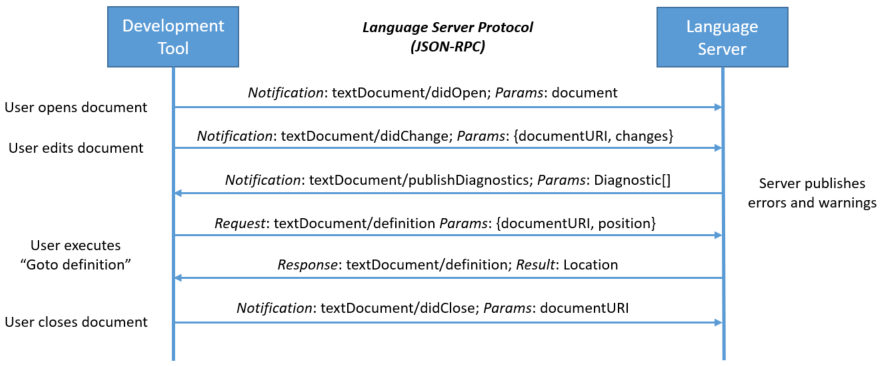
\includegraphics[height=0.4\linewidth]{Image/LSP-Diagram.png}
      \label{lsp-diagram}
      \footnotesize
      \\ Imagem não adaptada. \\
      Disponível em: \hyperlink{https://microsoft.github.io/language-server-protocol/overviews/lsp/overview/}{Microsoft - Language Server Protocol}
  \end{figure}
\end{frame}

\begin{frame}{Language Server Protocol - Instalação e Configuração}
  \textbf{Suporte nativo da API}
    \begin{columns}
      \begin{column}{0.4\textwidth}
        \begin{figure}
            \centering
            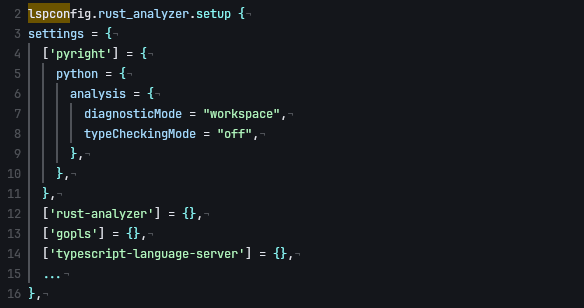
\includegraphics[height=0.6\linewidth]{Image/nvim-lspconfig.png}
            \label{nvim-lspconfig}
        \end{figure}
      \end{column}

      \begin{column}{0.6\textwidth}
        \begin{widedescription}
          \item Além de oferecer \textit{bindinds} nativas para a comunicação com LSPs, a configuração dos clientes pode
            ser feita de forma simples e direta através do pacote \texttt{nvim-lspconfig}
        \end{widedescription}
      \end{column}
  \end{columns}
\end{frame}

\begin{frame}{Language Server Protocol - Instalação e Configuração}
  \textbf{\texttt{nvim-lspconfig} + \texttt{Mason.nvim} = Configuração rápida, fácil, e portátil}
  \begin{figure}
      \centering
      
\includegraphics[height=0.3\linewidth]{Image/Mason-Logo.png}
      \label{mason-logo}
      \footnotesize
      \\ Imagem não adaptada. \\
      Disponível em:  \hyperlink{https://github.com/williamboman/mason.nvim}{Mason.nvim}
  \end{figure}
  \begin{quotation} \small
    Portable package manager for Neovim that runs everywhere Neovim runs. Easily install and manage LSP servers, DAP
    servers, linters, and formatters.\cite{masonNvim}
  \end{quotation}
\end{frame}

\begin{frame}{Language Server Protocol - Instalação e Configuração}
  \textbf{Um package-manager para servidores LSP}
  \begin{figure}
      \centering
      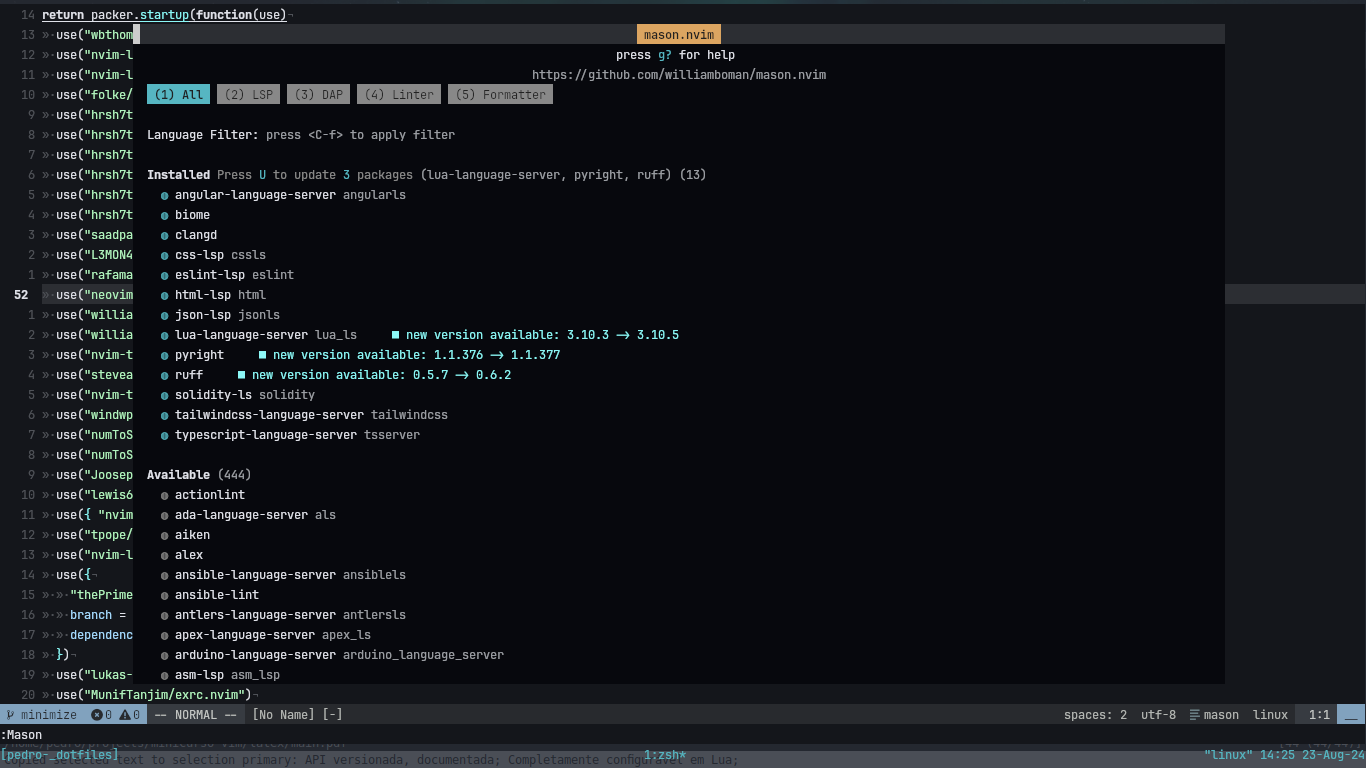
\includegraphics[height=0.5\linewidth]{Image/MasonLSP.png}
      \label{neovim-logo-2}
      \footnotesize
      \\ Instalação de LSPs via \textit{Mason.nvim} \\
  \end{figure}
\end{frame}

\begin{frame}{TreeSitter}
  \textbf{O motor sintático}
    \begin{columns}
      \begin{column}{0.3\textwidth}
        \begin{figure}
            \centering
            
\includegraphics[height=0.7\linewidth]{Image/TreeSitterLogo.png}
            \label{treesitter-logo}
        \end{figure}
      \end{column}

      \begin{column}{0.7\textwidth}
        \begin{widedescription}
          \item \begin{quotation} \small
            ``Tree-sitter is a parser generator tool and an incremental parsing library. It can build a
            concrete syntax tree for a source file and efficiently update the syntax tree as the source file is
            edited.''
          \end{quotation}
        \end{widedescription}
      \end{column}
  \end{columns}
\end{frame}

\begin{frame}{TreeSitter}
  \textbf{O motor sintático}
    \begin{widedescription}
      \item \textbf{General} enough to parse any programming language;
      \item \textbf{Fast} enough to parse on every keystroke in a text editor;
      \item \textbf{Robust} enough to provide useful results even in the presence of syntax errors;
      \item \textbf{Dependency-free} so that the runtime library (which is written in pure C) can be embedded in any application;
    \end{widedescription}
\end{frame}

\begin{frame}{TreeSitter}
  \textbf{O motor sintático}
    \begin{quotation} \small
      ``The goal of nvim-treesitter is both to provide a simple and easy way to use the interface for tree-sitter in
      Neovim and to provide some basic functionality such as highlighting based on it.''
    \end{quotation}
\end{frame}

\begin{frame}{TreeSitter}
  \textbf{O motor sintático}
  \begin{figure}
      \centering
      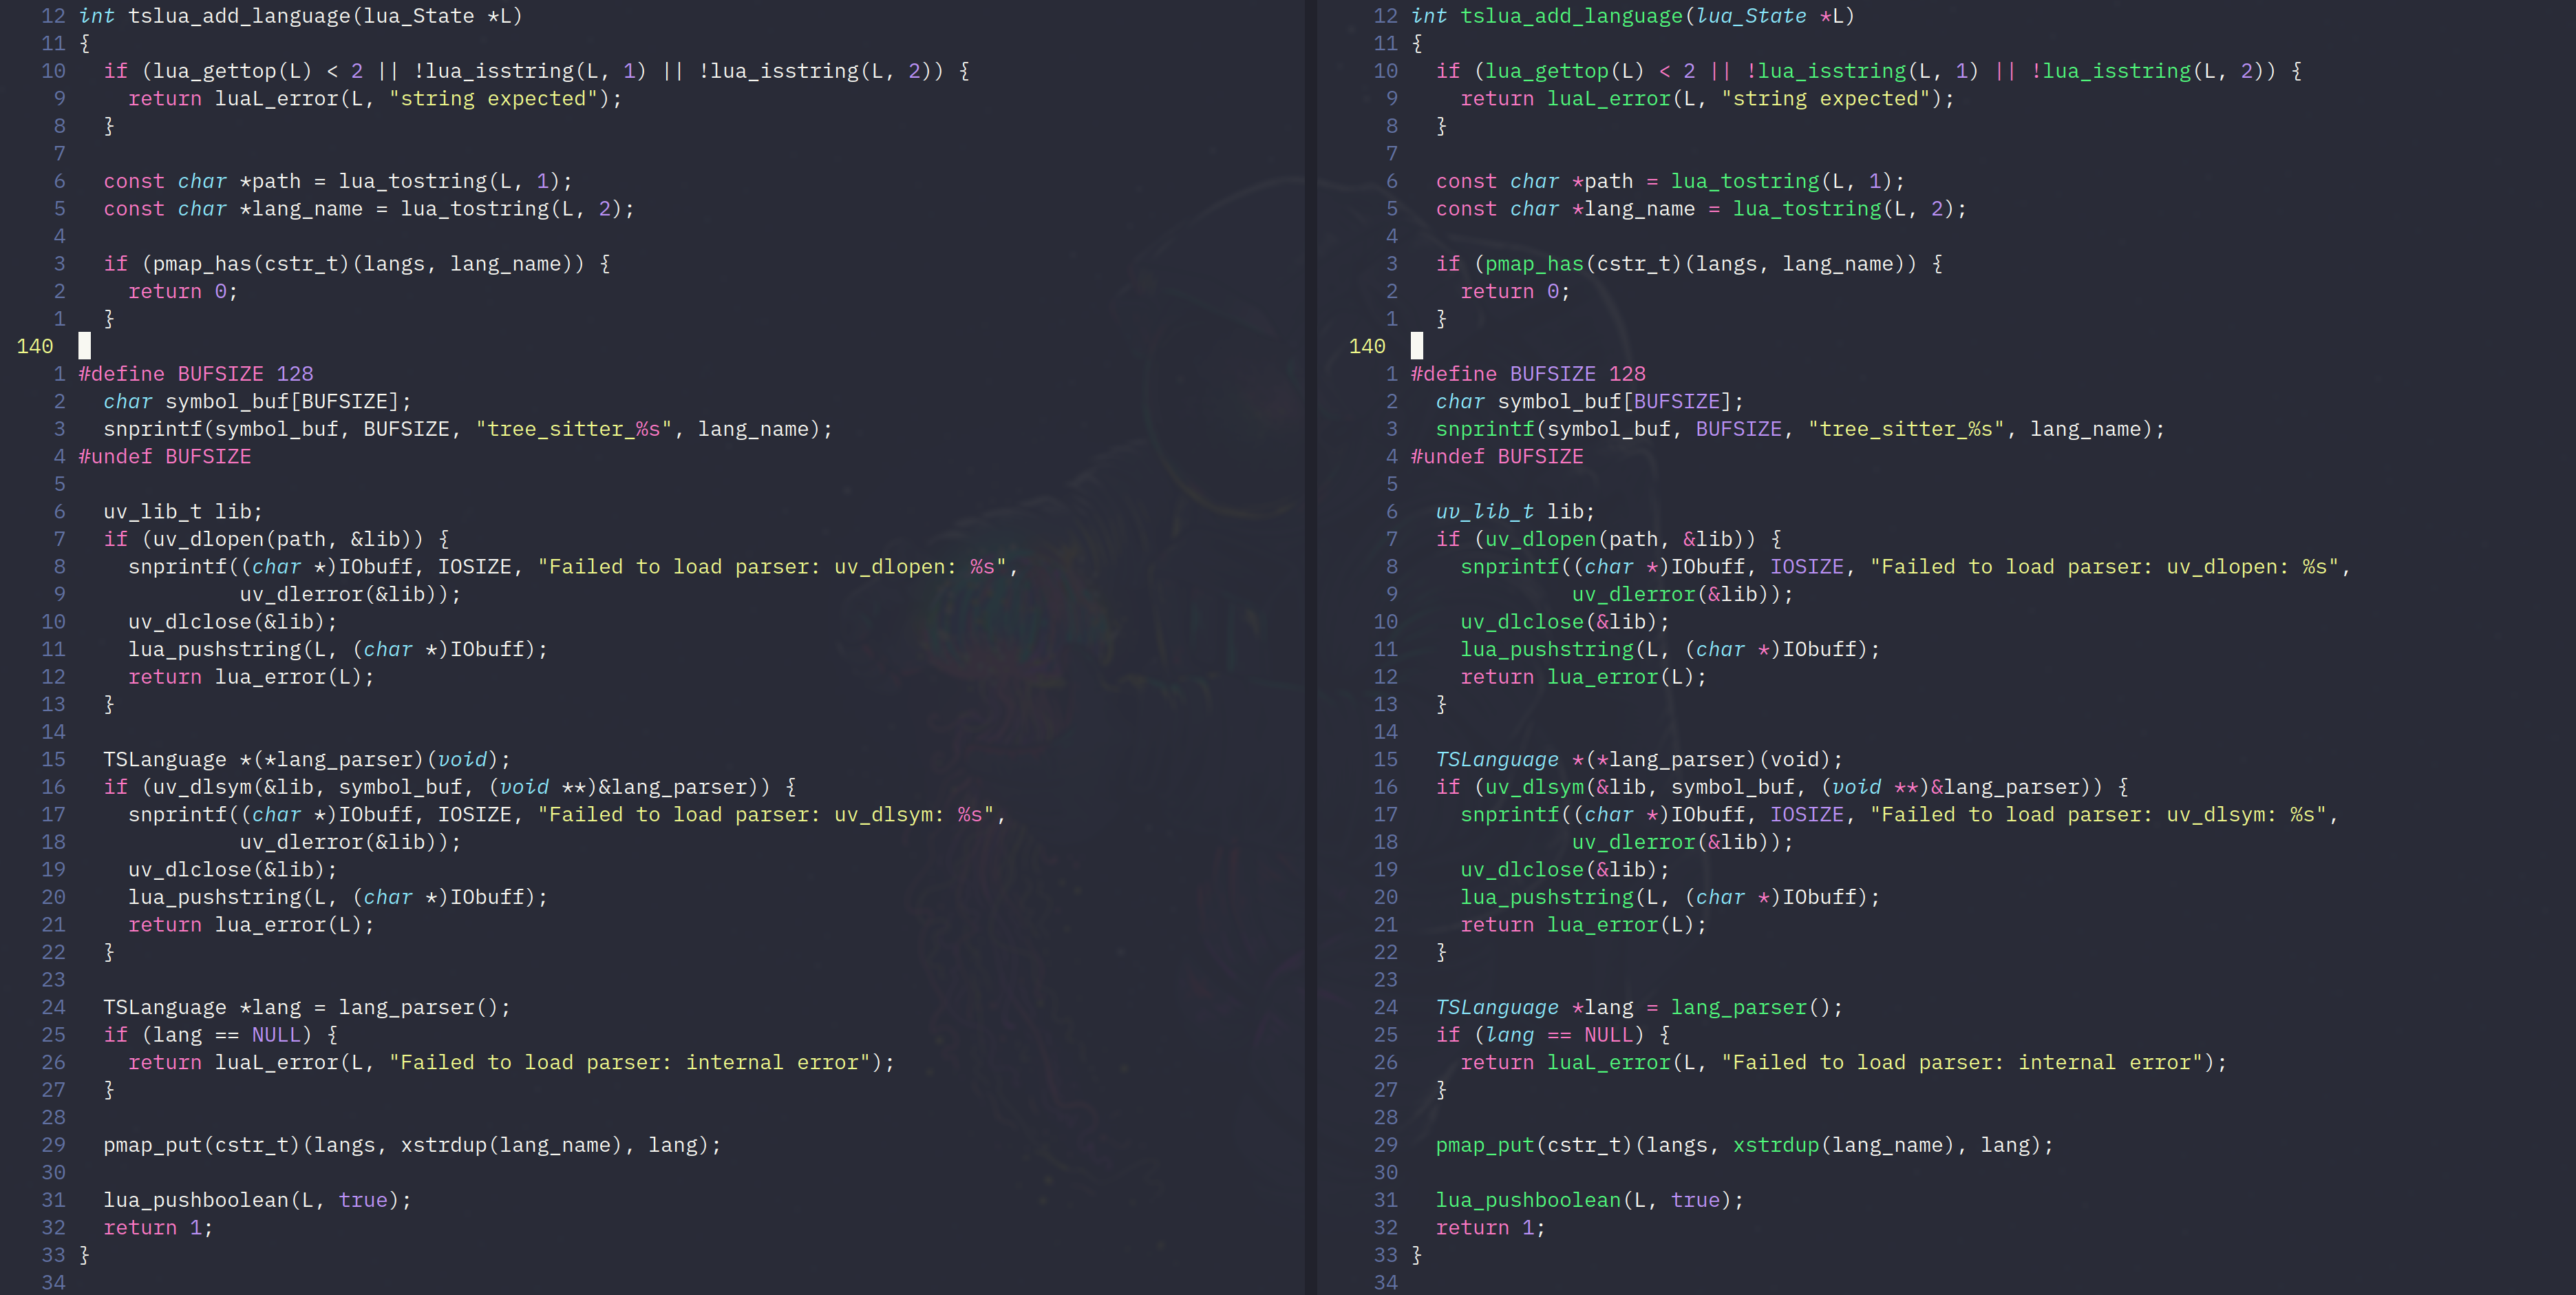
\includegraphics[height=0.5\linewidth]{Image/TreeSitter-Highlighting-Comparison.png}
      \label{treesitter-syntax-highlighting}
      \footnotesize
      \\ \textit{Highlighting} de sintaxe através da árvore construída\\
  \end{figure}
\end{frame}

\begin{frame}{TreeSitter}
  \textbf{O motor sintático}
  \begin{figure}
      \centering
      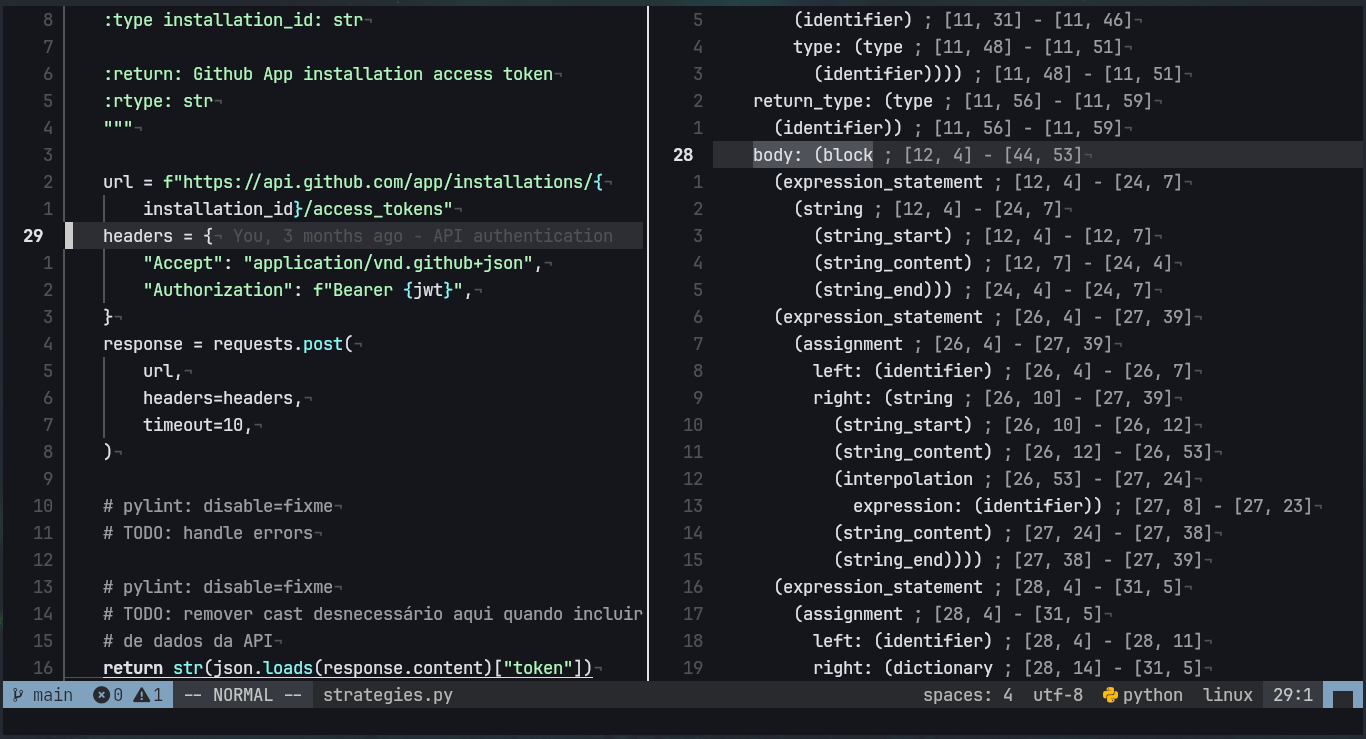
\includegraphics[height=0.5\linewidth]{Image/InspectTree.png}
      \label{treesitter-inspect-tree}
      \footnotesize
      \\ A ferramenta permite inspecionar a estrutura da árvore sintática em tempo real \\
  \end{figure}
\end{frame}

\begin{frame}{Plugins}
  \textbf{Plugin managers}
    \begin{widedescription}
      \item \texttt{pathogen}
      \item \texttt{vundle}
      \item \texttt{vim-plug}
      \item \texttt{packer.nvim}
      \item \textbf{\texttt{lazy.nvim}}
    \end{widedescription}
\end{frame}

\begin{frame}{Plugins}
  \textbf{Plugin managers}
  \begin{figure}
      \centering
      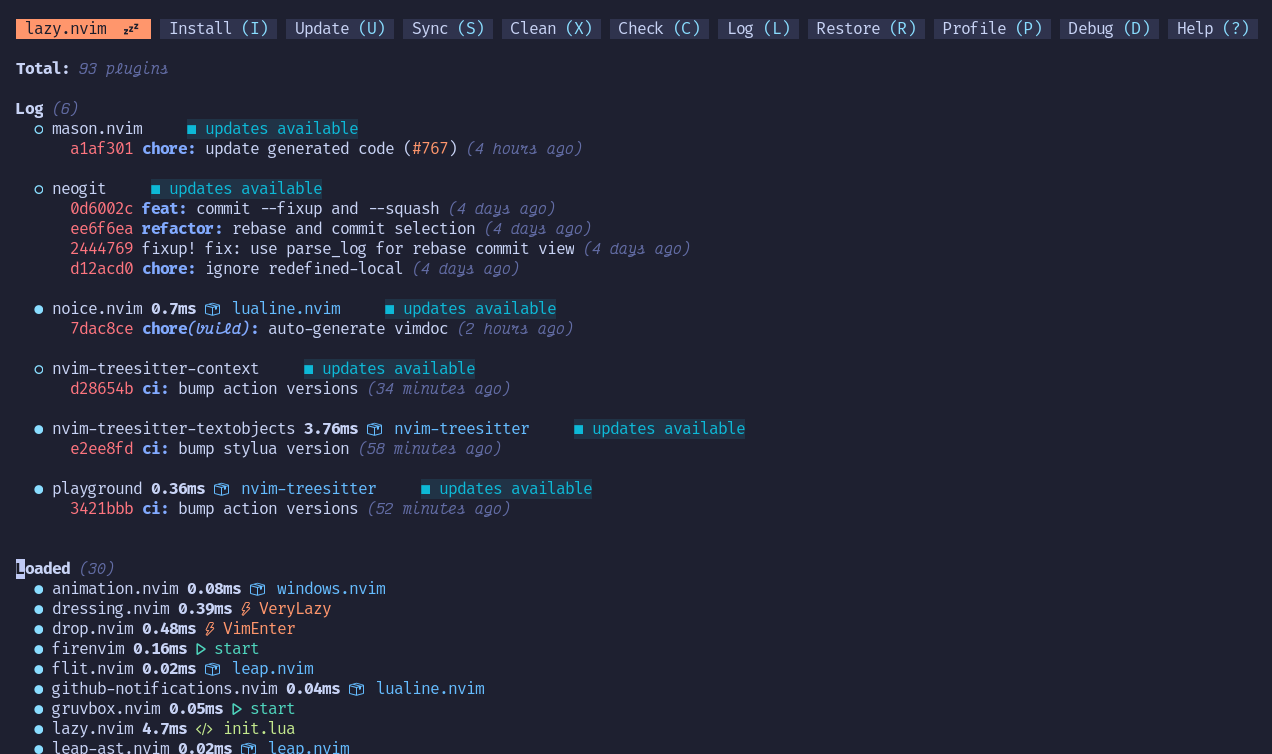
\includegraphics[height=0.5\linewidth]{Image/LazyVim.png}
      \label{lazy-vim}
      \footnotesize
      \\ Instalação interativa de plugins com \texttt{lazy.nvim} \\
  \end{figure}
\end{frame}

\begin{frame}{Lua}
  \textbf{Brasil mentioned!?!?!?}
  \begin{figure}
      \centering
      
\includegraphics[height=0.4\linewidth]{Image/Lua-Logo.png}
      \label{lua-logo}
      \footnotesize
      \\ Imagem não adaptada. \\
      Disponível em:  \hyperlink{https://www.lua.org/}{www.lua.org}
  \end{figure}
\end{frame}

\begin{frame}{Lua}
  \textbf{API}
    \begin{widedescription}
        \item The "Vim API" inherited from Vim: Ex-commands and builtin-functions as
          well as user-functions in Vimscript. These are accessed through \texttt{vim.cmd()}
          and \texttt{vim.fn} respectively.
        \item The "Nvim API" written in C for use in remote plugins and GUIs; see api.
          These functions are accessed through \texttt{vim.api}.
    \end{widedescription}
\end{frame}

\section{Encerramento}
\begin{frame}{Recomendações}
    \hyperlink{https://vim-adventures.com/}{vim-adventures.com}

    \vfill
    
    \fbox{
        \parbox{\linewidth}{
        \$ vimtutor
        }
    }

    \vfill

    \key{:help}
\end{frame}

\begin{frame}[t]{Referência}
    \nocite{*}
    \bibliographystyle{amsalpha}
    \bibliography{references}
\end{frame}


\end{document}

%\section{Introdução}
%
%    
%    \begin{frame}{Terminal}
%        \fbox{
%            \parbox{\linewidth}{
%            \textbf{user}@hostname \~\ \%    
%            }
%        }
%        
%        \fbox{
%            \parbox{\linewidth}{
%            \textbf{user}@hostname \~\ \%    
%            }
%        }
%    \end{frame}
%
%\section{Navegação}
%    \begin{frame}{Comandos}
%        \begin{itemize}
%            \item ls: Lista arquivos e diretórios
%
%            \item cd: Muda de diretório
%
%            \item pwd: Mostra o diretório atual
%        \end{itemize}
%    \end{frame}
%
%    \begin{frame}{Flags}
%        Flags comuns para ls:
%        \begin{itemize}
%            \item -l (long listing):     detalhado
%            \item -h (--human-readable): mais "legível"
%            \item -S (Sort by size):     ordena por tamanho
%            \item -t (sort by time):     ordena por tempo
%            \item -r (--reverse):        ordena na ordem reversa
%            \item -a (--all):            mostra entradas ocultas
%        \end{itemize}
%    \end{frame}
%
%    \begin{frame}{Diretórios}
%
%        Arquivos e diretórios ocultos
%        
%        Diretórios . .. \~\ 
%        
%    \end{frame}
%
%    \begin{frame}{Gerência de arquivos}
%        \begin{itemize}
%            \item mkdir (make directories): cria diretórios. 
%            \item mv: move (rename) arquivos
%            \item cp: copia arquivos e diretórios
%            \item rm: remove arquivos e diretórios
%        \end{itemize}
%    \end{frame}
%
%\section{Entrada e saída}
%
%    \begin{frame}
%        \includegraphics[width=\textwidth, page=2]{Image/Imagens para minicurso Linux.pdf}
%    \end{frame}
%
%    \begin{frame}{Manipulação}
%        Para manipular entrada e saída temos os seguintes operadores.
%        
%        \begin{itemize}
%            \item \textless: Coloca um arquivo na entrada padrão.
%            \item \textgreater: Redireciona saída padrão para um arquivo.
%            \item 2\textgreater: Redireciona saída de erro para um arquivo.
%            \item \&\textgreater: Redireciona saída padrão e de erro para um arquivo.
%            \item \textgreater\textgreater: Concatena saída padrão a um arquivo.
%            \item $\vert$ : Redireciona saída de um comando para entrada de outro.
%        \end{itemize}
%    \end{frame}
%
%\section{Comandos}
%    \begin{frame}{Visualização de texto}
%        \begin{itemize}
%            \item cat: concatena arquivos para a saída padrão
%            \item more: para visualizar um arquivo cada vez mais
%            \item less: o oposto de more
%            \item head: para visualizar o começo de um arquivo
%            \item tail: para visualizar o final de um arquivo
%            \item grep (\textbf{globally} search for a \textbf{regular expression} and \textbf{print} matching lines): busca por padrões 
%        \end{itemize}
%
%        * A flag -n controla o número de linhas no comando head e tail.
%    \end{frame}
%
%    \begin{frame}{Utilitários}
%        \begin{itemize}
%            \item echo: "ecoa" o texto passado
%            \item man: consulta o manual de um programa
%            \item du (device usage): estima o espaço utilizado por um arquivo
%            \item df (disk free): reporta o espaço utilizado por um sistema de arquivo
%        \end{itemize}
%    \end{frame}
%
%    \begin{frame}{Empacotador de arquivos}
%        tar (tape archive): compactar e descompactar arquivos
%        \begin{itemize}
%            \item -c (--create): cria um arquivo
%            \item -t (--list): lista um arquivo
%            \item -x (--extract, --get): extrai um arquivo
%            \item -z (--gzip): comprime/extrai com gzip
%            \item -j (--bzip2): comprime/extrai com bzip2
%            \item -f (--file=ARCHIVE): especifica arquivo
%        \end{itemize}
%    \end{frame}
%
%    \begin{frame}{Controle de processos}
%        \begin{itemize}
%            \item ps: lista processos no instante atual
%            \item top: lista processos em tempo real
%            \item jobs: lista processos em segundo plano
%            \item kill: mata um processo
%            \item pkill: mata um processo baseado no nome
%        \end{itemize}
%    \end{frame}
%
%    \begin{frame}{Sinais}
%        \begin{itemize}
%            \item SIGTSTOP (Ctrl + Z): pausa a execução (não pode ser ignorado)
%            \item SIGINT (Ctrl + C): Interrompe a execução
%            %\item SIGQUIT: Ctrl + \textbackslash
%            \item SIGKILL (-9): mata a execução (não pode ser ignorado)
%        \end{itemize}
%    \end{frame}
%
%    \begin{frame}{Gerência de tarefas}
%        \begin{itemize}
%            \item bg (background): executa o processo em segundo plano
%            \item fg (foreground): executa o processo em primeiro plano
%            \item disown: desvincula o processo do shell
%            \item \&: inicia o processo em segundo plano
%        \end{itemize}
%    \end{frame}
%
%\section{Permissão}
%
%    \begin{frame}{Bits de permissão}
%        \begin{itemize}
%            \item r (readable): permissão de leitura
%            \item w (writeable): permissão de escrita
%            \item x (executable): permissão de execução
%        \end{itemize}
%    \end{frame}
%
%    \begin{frame}{Alterar permissão}
%        \begin{itemize}
%            \item chmod (change file mode bits): altera permissões do arquivo
%            \item chown (change file owner and group): altera dono do arquivo
%        \end{itemize}
%    \end{frame}
%
%    \begin{frame}{Exemplo}
%        hello.sh
%        \fbox{
%            \parbox{\textwidth}{
%                \#!/bin/bash \\
%                echo "Hello, world"
%            }
%        }
%    \end{frame}
%
%    \begin{frame}{Super usuário}
%        \begin{itemize}
%            \item su (substitute user): alterar usuário
%            \item sudo (substitute user do): executa comando como outro usuário
%        \end{itemize}
%    \end{frame}
%
%\section{Conclusão}
%    \begin{frame}{Dúvidas?}
%        \begin{center}
%            \includegraphics[scale=0.13]{Image/Tux.svg.png}
%        \end{center}
%    \end{frame}
